\newpage

%TODO Si travail en mode agile, inclure une analyse de la méthode de travail, (identifier ce qui était prévu au départ au niveau macro, l'implémentation effective, les virages pris après chaque sprint après les retours clients).

\section{Gestion de projet}
\label{sec:projectManagement}

\subsection{Méthode de travail employée}
La méthode de travail utilisée est proche de la méthode Scrum.
\paragraph*{Les sprints\\}
Le projet est découpé en "Sprints". Un sprint est une période de temps donnée, durant laquelle un certain nombre de fonctionnalités doivent être implémentées par les développeurs. A la fin de la période, le travail réalisé est présenté au client.\\

La méthode Scrum recommande des sprints d'une durée d'environ deux semaines. Cependant, dans le cadre de notre projet, les sprint ont plutôt une durée comprise entre un et deux mois. Cela se justifie notamment par le fait que certaines fonctionnalités peuvent avoir un temps de développement long.\\
Le fait que la durée soit plus longue que celle recommandée présente des intérêts et des désavantages. 
Un sprint plus long permet de solliciter le client moins souvent, de limiter le temps alloué à la gestion du sprint lui même, de limiter le nombre de rendus.
Le point négatif d'une durée allongée est que cela limite le nombre de retours clients et augmente ainsi le risque d'une inadéquation entre le travail réalisé et l'attendu.

\paragraph*{Les stand-up meetings\\}
La méthode Scrum introduit le concept de "Mêlée quotidienne" (aussi appelé "daily scrum" ou "stand-up meeting")\cite{bib:dailyScrum}.\\
D'après les recommandations de la méthode, ce type de réunion doit être de courte durée (15 minutes), se dérouler de préférence le matin et aborder trois questions :
\begin{sitemize}
	\item Quel travail a été effectué la veille ?
	\item Quel travail sera réalisé dans la journée ?
	\item Y a-t-il des obstacles qui empêchent la réalisation des objectifs fixés ?
\end{sitemize}

Dans le cadre du projet, des stand-up meetings sont réalisés à raison d'une fois par semaine environ. Ces réunions permettent à l'équipe d'être au courant de ce que chacun fait et n'ont pas pour but de résoudre des problèmes.\\
Lorsqu'un problème se pose, il est généralement discuté directement entre le chef de projet et le développeur qui y est confronté.

\paragraph*{La planification des sprints\\}
Dans la méthode Scrum, la planification a lieu en équipe\cite{bib:springPlanning}, avec le "\textit{product owner}"\footnote{product owner (propriétaire du produit): Il s'agit de la personne qui fait le lien entre la maitrise d'ouvrage et la maitrise d'oeuvre.}. \\
Durant cette réunion, le product owner doit apporter le "\textit{product backlog}"\footnote{product backlog (carnet de produit): il contient la liste ordonnée des besoins et fonctionnalités à implémenter dans la suite du projet.} et décider avec l'équipe quels seront les objectifs du sprint.\\
Durant la réunion, certaines "\textit{user-stories}" du product backlog sont choisies et découpées en tâches détaillées. A l'issue de la réunion, l'équipe repars avec le "\textit{sprint backlog}". Le \textit{sprint backlog} contient la liste des \textit{user-stories} que l'équipe s'est engagé à livrer et la liste des tâches à réaliser pour y parvenir.\\

Du fait de l'activité d'édition logiciel, sur le projet, la planification du sprint est discutée entre le directeur de l'entreprise et le chef de projet. Par la suite, le chef de projet établis le \textit{sprint backlog}, et le transmet à l'équipe (via \textit{Jira}).

\paragraph*{La réunion de présentation du sprint\\}
Dans la méthode Scrum, il s'agit du \textit{Sprint Review Meeting}. Le but de la réunion est de présenter le travail réalisé pendant le sprint. 

Dans le cadre du projet, cette réunion sert à faire la démonstration au client des fonctionnalités implémentées et à aborder la suite du projet.\\
C'est également l'occasion pour le client de faire un retour sur le travail réalisé.

%TODO OK Méthode de travail employée : méthode de développement, mode de travail en équipe, réunions-présentations etc.

\subsection{Outils d'assistance au développement utilisés.}
Pour réaliser la gestion du projet, nous utilisons l'outil \textit{Jira}.
Jira permet de découper les fonctionnalités à réaliser en tâches et de les affecter ensuite aux membres du projet.\\
Au fur et à mesure que le projet avance, chaque développeur journalise le nombre d'heures qu'il a travaillé sur chaque tâche et fait évoluer leur statut (tâche ouverte, en cours, en cours de revue, finie).\\
L'utilité de Jira est donc double puisqu'il permet à la fois de planifier le projet, mais également de suivre son avancement. La maitrise d'oeuvre s'en sert donc pour s'organiser et la maitrise d'ouvrage l'utilise pour se tenir au courant de l'avancement des travaux.\\

Le deuxième outil utilisé par l'équipe est \textit{Confluence}. Il permet de partager et gérer les documents propres au projet. De plus, Il offre une gestion de version et l'aperçu instantané des documents. On l'utilise pour stocker la documentation fonctionnelle, la documentation technique, l'architecture du projet, et le manuel utilisateur.\\

Enfin, pour l'hébergement du code du projet, nous utilisons \textit{Bitbucket} associé à\textit{Git}. \textit{Bitbucket} permet d'héberger le projet sur un répertoire privé. \textit{Git} permet de gérer les différentes versions du projet et de mettre en commun le travail réalisé par les développeurs. 

%TODO Outils d'assistance au développement utilisés.

\newpage
\subsection{Planning prévisionnel et réalisé} % (2 pages) Diagramme de gant avec planning prévisionnel
\paragraph*{Sprint 2}
\subparagraph{Objectifs globaux}
Le second sprint du projet a commencé en début mars, peu de temps après mon arrivée. Il a été dimensionné pour tenir sur 7 semaines.\\
Les objectifs de ce sprint portent sur la création des fonctionnalités suivantes : 
\begin{itemize}
	\item \textit{La gestion des patients} : ajouter les FSE (Feuilles de Soins Electroniques) : Il s'agit des feuilles de soins qui sont créées par le praticien et qui décrivent la prise en charge du bénéficiaire des soins ainsi que les différents actes réalisés et leur coût. La \gls{FSE} est mise à jour avec la carte vitale du patient à la réalisation du dernier acte et est ensuite transmise à l'assurance maladie.
	
	\item \textit{Les factures et la télé-transmission} : mettre en place le contexte de facturation. Le contexte comprend la gestion des tarifications, des types de couverture et des types de prise en charge. Cette fonctionnalité nécessite la lecture des cartes SESAM Vitale.

	\item \textit{Le dossier médical} : démarrer la fonctionnalité. Le dossier médical contient une liste des documents associés au patient (ordonnances, factures, prescriptions, scans, images etc.)
	
	\item \textit{La gestion des ordonnances} : ajouter les cas métiers de la gestion des séances. La gestion de base des séances faisait partie du sprint 1. Dans ce sprint ce sont les cas particuliers (i.e. les cas de figure issus du terrain) qui sont traités. Ces cas de figure couvrent par exemple l'annulation ou le décalage d'une séance par le praticien ou le client.

	\item \textit{L'intégration continue et le TDD} : Ce n'est pas une fonctionnalité à proprement parlé, mais plus une amélioration des méthodes de production. L'intégration continue doit permettre une industrialisation de la production (tests lancés automatiquement lors du build et obtention de rapports portants sur la qualité du code). La méthodologie de TDD\footnote{TDD: Test-Driven Development (Développement dirigé par les tests).} porte sur la façon de développer et tester le logiciel. Elle doit permettre d'augmenter la qualité du code développé.
\end{itemize}

\subparagraph{Objectifs personnels}
En ce qui me concerne, durant ce sprint, je devais implémenter les fonctionnalités de base du dossier médical (liste des documents), intégrer un éditeur de textes et concevoir une galerie d'images.\\
Voici le diagramme de Gantt prévisionnel et le gantt effectif : 
\begin{figure}[H]
  \centering
  \centerline{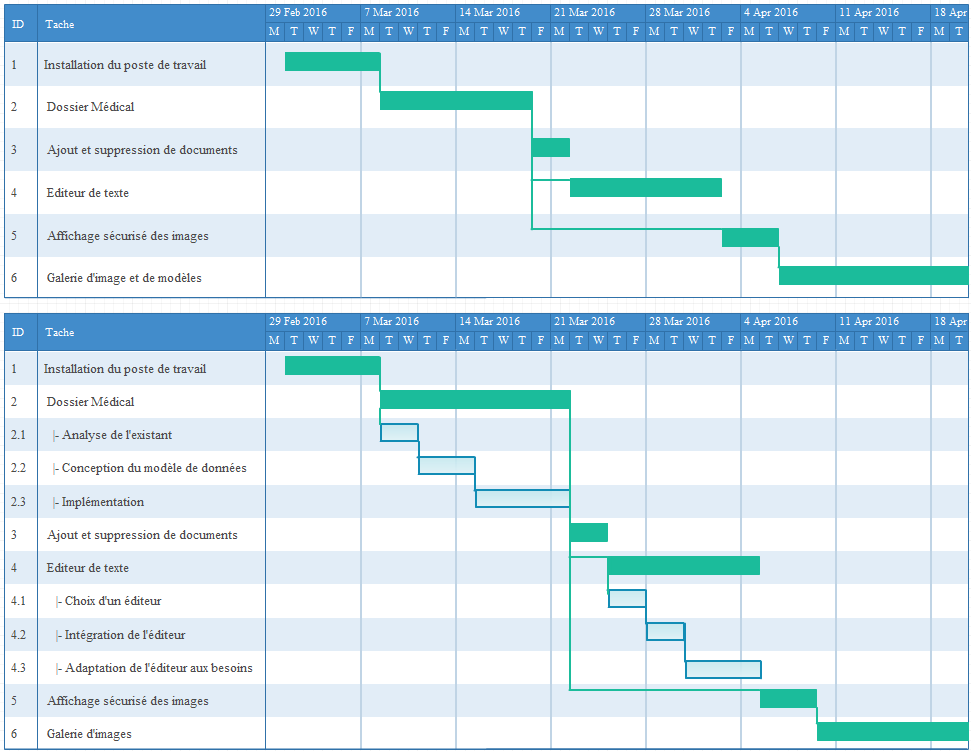
\includegraphics[width=20.5cm]{./img/gantt_sprint2}}
  \caption{\label{fig:mb_va_ast} Gantt prévisionnel et Gantt réalisé du Sprint 2.}
\end{figure}
Le sprint s'est déroulé globalement comme prévu. L'implémentation du dossier médical a pris un peu plus de temps que prévu, car il m'a fallu un moment pour découvrir les technologies et les méthodes de travail de l'équipe.

\newpage
\paragraph*{Sprint 3\\}
Ce troisième sprint prend place du 18 Avril au 23 Mai.\\ 
Il était prévu que durant cette période, nous travaillions en collaboration avec des ergonomes et des designers afin d'améliorer l'expérience utilisateur. \\
Dans les faits, la prise de contact avec le cabinet d'ergonomes a bien eu lieu, mais l'étude de l'ergonomie du logiciel prend un certain temps. De ce fait, les modifications concernant l'expérience utilisateur et le design ne se feront pas pendant ce sprint.

\subparagraph{Objectifs globaux}
L'objectif du sprint est de faire avancer le projet sur quatre domaines : 
\begin{itemize}
\item \textit{La gestion des patients} : Ajouter la possibilité de créer manuellement un patient et de synchroniser le dossier d'un patient avec sa carte vitale.

\item \textit{Les factures et la télétransmission} :
Création des DRE (Demandes de remboursement electroniques)

\item \textit{Le dossier médical} : Ajouter la gestion des modèles de documents et des placeholders.

\item \textit{La gestion des ordonnances} : Ajouter la saisie d'une DAP \footnote{DAP: Demande d'accord préalable. Les DAP concernent les rééducations en masso-kinésithérapie. Pour chaque type de rééducations, il est prévu qu'un certain nombre de séances soient remboursées par la sécurité sociale. Si ce nombre de séances doit être dépassé, il convient de faire une demande préalable (la DAP).}. Prise en compte des natures d'assurance\footnote{Il existe plusieurs natures d'assurance: maladie, accident du travail, maternité. La nature d'assurance impacte le taux de prise en charge.}
\end{itemize} 

\subparagraph{Objectifs personnels :}
Mon objectif durant ce sprint était de compléter la fonctionnalité d'édition de texte du dossier médical, en ajoutant les champs génériques et les modèles de documents.\\
Il était également prévu que je revoie l'authentification à l'API Sésame, pour y introduire le concept de postes utilisateurs. Cette fonctionnalité a été prévue dans l'optique de pouvoir ajouter la fonction de numérisation dans le sprint 4.

\begin{figure}[H]
  \centering
  \centerline{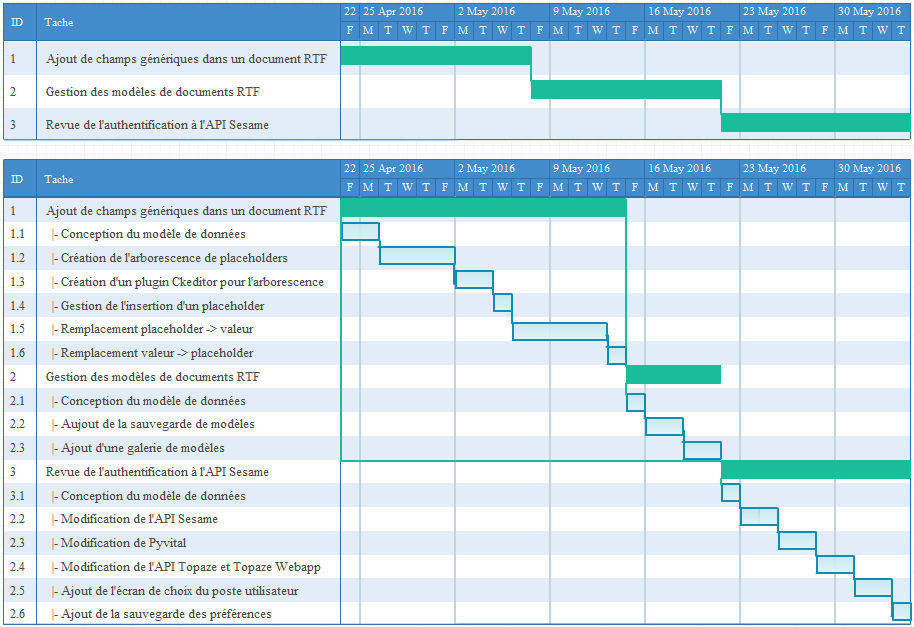
\includegraphics[width=20.5cm]{./img/gantt_sprint3}}
  \caption{\label{fig:mb_va_ast} Gantt prévisionnel et Gantt réalisé du Sprint 3.}
\end{figure}

Durant ce sprint, la fonctionnalité principale était l'ajout des champs génériques. Cette tâche était intéressante techniquement car elle m'a fait découvrir l'introspection de java. Cette tâche a pris un certain temps car elle a demandé un effort de conception particulier lors de la création de l'arborescence de placeholders et les 3 phases de remplacements des champs génériques par leurs valeurs.  \\
L'ajout des modèles de documents a été implémenté plus rapidement que prévu grâce aux composants réutilisables que j'ai créé en sprint 2.\\
La tâche de 

\newpage
\paragraph*{Sprint 4}
\subparagraph{Objectifs globaux}

Les objectifs du sprint 4 sont : 
\begin{itemize}
\item \textit{La gestion des patients} : ajout  de la prise en compte des maternités et arrêts de travail dans la fiche patient.

\item \textit{Les factures et la télé-transmission} : ajout de la recherche de conventions. \footnote{Les conventions: Les médecins signent des conventions avec des mutuelles ou des regroupements de mutuelles et peuvent ensuite émettre des demandes de remboursement électronique.} 
%(praticien et une amc ou regroupement de mutuelles) recherche convention gestion unique ou séparée, transmission de DRE dans le cas des tiers payants)

\item \textit{Le dossier médical} : Ajout de la fonctionnalité de numérisation et de la possibilité de traiter l'image obtenue (crop, rotation ...).

\item \textit{La gestion des ordonnances} : Ajout de la DSI (Démarche de Soin Infirmier).

\item \textit{Autre} : Création d'un installateur windows pour le driver Pyvital. 
\end{itemize} 

\subparagraph{Objectifs personnels}
Durant ce sprint, j'ai continué à travailler sur le dossier médical. Mon objectif était cette fois d'ajouter la fonctionnalité de numérisation. \\
D'autre part, dans l'optique d'une commercialisation qui approche, j'ai eu à implémenter un installateur pour le driver Pyvital. 
\begin{figure}[H]
  \centering
  \centerline{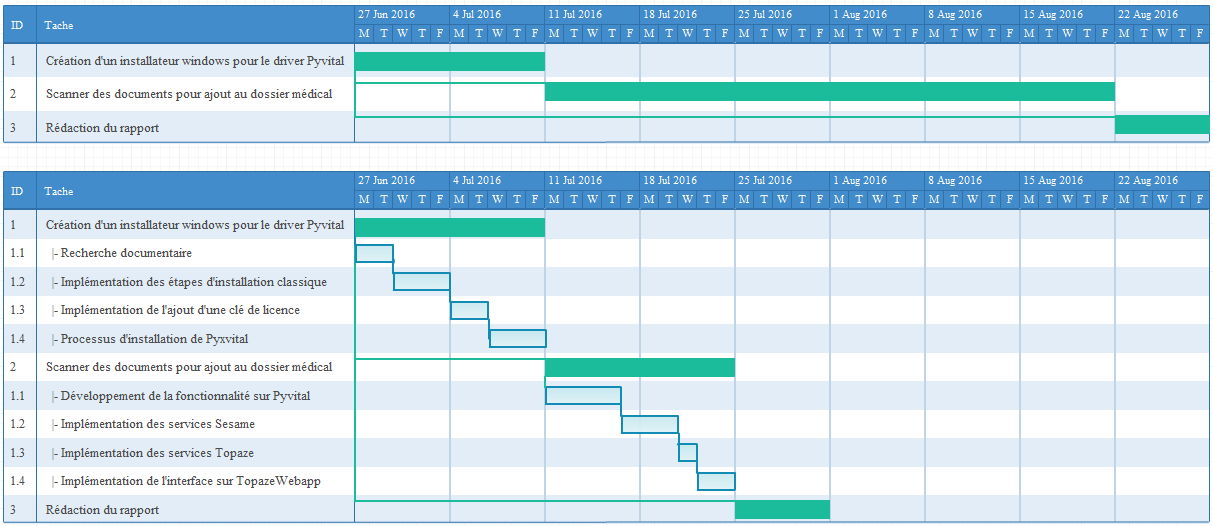
\includegraphics[width=20.5cm]{./img/gantt_sprint4}}
  \caption{\label{fig:mb_va_ast} Gantt prévisionnel et Gantt réalisé du Sprint 4.}
\end{figure}

\paragraph*{Rétrospective et vision future\\}
Après le sprint 4, le projet offrira les fonctionnalités de base pour gérer un cabinet et créer les documents médicaux.
Voici le récapitulatif, par domaine, de l'état du projet et des fonctionnalités envisagées par la suite.
\begin{itemize}
	\item \textit{La gestion des patients} : le logiciel offre désormais la possibilité de créer des patients, de mettre à jour leurs informations avec la carte vitale et de générer des feuilles de soins électroniques.
	Dans le futur, le logiciel devra être capable d'assurer le suivi des factures et des règlements.
	
	\item \textit{Les factures et la télé-transmission} : aujourd'hui, le logiciel est capable de créer des feuilles de soins électroniques et des demandes de soins électroniques. Par la suite, ces documents électroniques devront pouvoir être mis en lots et transmis aux organismes. Il faudra également traiter les ARL (Accusé de Réception Logique) reçus après les transmissions.
	%(praticien et une amc ou regroupement de mutuelles) recherche convention gestion unique ou séparée, transmission de DRE dans le cas des tiers payants)
	
	\item \textit{Le dossier médical} : le dossier médical permet à un praticien (kinésithérapeute ou infirmier) de gérer les documents liés à ses patients, de créer des documents textes et de scanner des documents. Par la suite, il faudra également gérer le dossier médical des sages-femmes qui présente des particularités propres au métier.
	
	\item \textit{La gestion des ordonnances} : il est aujourd'hui possible de créer des ordonnances (pour les kinésithérapeutes et infirmiers), de gérer des séances et de créer des DAP. Par la suite, les kinés devra pouvoir effectuer un bilan des soins effectués et une sage-femme devra pouvoir faire un suivi de grossesse.
	
	\item \textit{Les SCORs} : l'application devra pouvoir créer et émettre des SCOR (SCans d'ORdonnances). Ce sont des ordonnances numérisées dont le formatage respecte une certaine norme.
\end{itemize} 

%TODO Planning prévisionnel 
%TODO Planning réalisé + explications

%TODO définition des tâches 
%TODO Différences prévisionnel/réalisé
%TODO Tâches particulières

\subsection{Évaluation du coût du projet réalisé\\}
Le coût du projet réalisé durant le stage est à ce jour (25 Juillet) de 90 Jour-Hommes.
%TODO Faites une évaluation du coût du projet que vous avez réalisé (en environné), si besoin faites vous aider par votre tuteur en entreprise. 